\documentclass{standalone}
\usepackage{tikz}
\usetikzlibrary{patterns, positioning}
\usepackage[sfdefault]{ClearSans} %% option 'sfdefault' activates Clear Sans as the default text font
\usepackage[T1]{fontenc}

\begin{document}
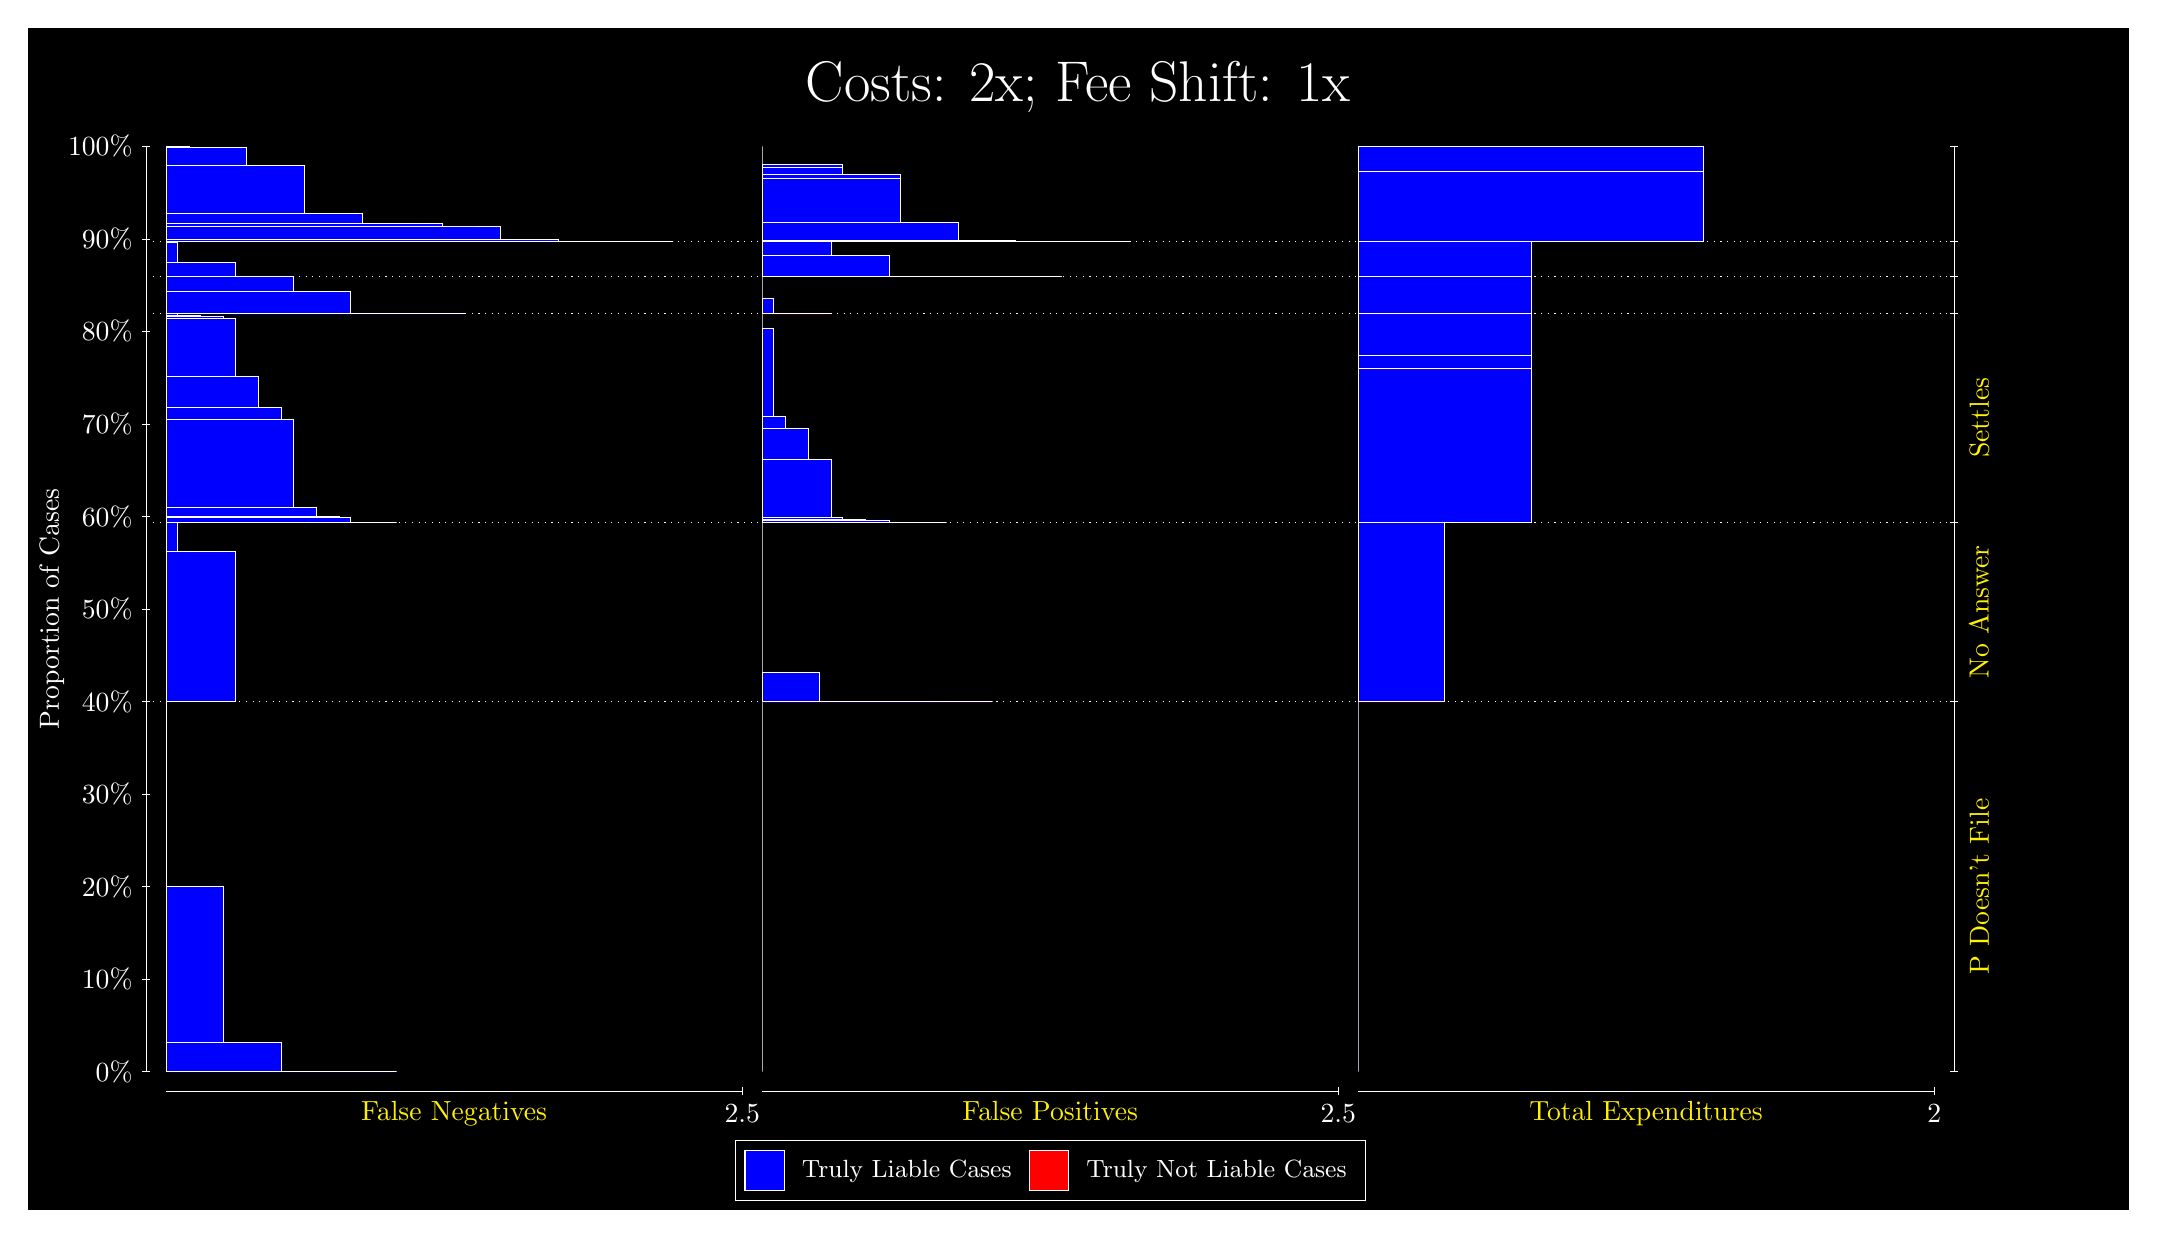
\begin{tikzpicture}
\draw[fill=black] (0,0) rectangle (26.667,15);
\draw[text=white] (0,13.5) rectangle (26.667,15) node[midway] {\huge Costs: 2x; Fee Shift: 1x};
\draw[white, very thin] (1.5,1.75) -- (1.5,13.5);
\node[rotate=90, text=white, anchor=center] at (0.3, 7.625) {Proportion of Cases};
\draw[white, very thin] (1.45,1.75) -- (1.55,1.75);
\node[text=white, anchor=east] at (1.45, 1.75) {0\%};
\draw[white, very thin] (1.45,2.925) -- (1.55,2.925);
\node[text=white, anchor=east] at (1.45, 2.925) {10\%};
\draw[white, very thin] (1.45,4.1) -- (1.55,4.1);
\node[text=white, anchor=east] at (1.45, 4.1) {20\%};
\draw[white, very thin] (1.45,5.275) -- (1.55,5.275);
\node[text=white, anchor=east] at (1.45, 5.275) {30\%};
\draw[white, very thin] (1.45,6.45) -- (1.55,6.45);
\node[text=white, anchor=east] at (1.45, 6.45) {40\%};
\draw[white, very thin] (1.45,7.625) -- (1.55,7.625);
\node[text=white, anchor=east] at (1.45, 7.625) {50\%};
\draw[white, very thin] (1.45,8.8) -- (1.55,8.8);
\node[text=white, anchor=east] at (1.45, 8.8) {60\%};
\draw[white, very thin] (1.45,9.975) -- (1.55,9.975);
\node[text=white, anchor=east] at (1.45, 9.975) {70\%};
\draw[white, very thin] (1.45,11.15) -- (1.55,11.15);
\node[text=white, anchor=east] at (1.45, 11.15) {80\%};
\draw[white, very thin] (1.45,12.325) -- (1.55,12.325);
\node[text=white, anchor=east] at (1.45, 12.325) {90\%};
\draw[white, very thin] (1.45,13.5) -- (1.55,13.5);
\node[text=white, anchor=east] at (1.45, 13.5) {100\%};

\draw[white, very thin] (24.457,1.75) -- (24.457,13.5);
\draw[white, very thin] (24.407,1.75) -- (24.507,1.75);
\node[anchor=west] at (24.407, 1.75) {};
\draw[white, very thin] (24.407,6.4489) -- (24.507,6.4489);
\node[anchor=west] at (24.407, 6.4489) {};
\draw[white, very thin] (24.407,8.7281) -- (24.507,8.7281);
\node[anchor=west] at (24.407, 8.7281) {};
\draw[white, very thin] (24.407,11.375) -- (24.507,11.375);
\node[anchor=west] at (24.407, 11.375) {};
\draw[white, very thin] (24.407,11.847) -- (24.507,11.847);
\node[anchor=west] at (24.407, 11.847) {};
\draw[white, very thin] (24.407,12.294) -- (24.507,12.294);
\node[anchor=west] at (24.407, 12.294) {};
\draw[white, very thin] (24.407,13.5) -- (24.507,13.5);
\node[anchor=west] at (24.407, 13.5) {};

\draw[white, very thin, fill=blue] (1.75,1.75) rectangle (4.6775,1.75);
\draw[white, very thin, fill=blue] (1.75,1.75) rectangle (3.9457,1.7532);
\draw[white, very thin, fill=blue] (1.75,1.7532) rectangle (3.2138,2.126);
\draw[white, very thin, fill=blue] (1.75,2.126) rectangle (2.4819,4.1027);
\draw[white, very thin, fill=red] (1.75,4.1027) rectangle (1.75,4.1027);
\draw[white, very thin, fill=blue] (1.75,4.1027) rectangle (1.75,6.4489);
\draw[white, very thin, fill=blue] (1.75,6.4489) rectangle (2.6283,8.3557);
\draw[white, very thin, fill=blue] (1.75,8.3557) rectangle (1.8964,8.7254);
\draw[white, very thin, fill=red] (1.75,8.7254) rectangle (1.75,8.7254);
\draw[white, very thin, fill=blue] (1.75,8.7254) rectangle (1.75,8.7281);
\draw[white, very thin, fill=blue] (1.75,8.7281) rectangle (4.6775,8.7281);
\draw[white, very thin, fill=blue] (1.75,8.7281) rectangle (4.3848,8.7284);
\draw[white, very thin, fill=blue] (1.75,8.7284) rectangle (4.092,8.7907);
\draw[white, very thin, fill=blue] (1.75,8.7907) rectangle (3.9457,8.7978);
\draw[white, very thin, fill=blue] (1.75,8.7978) rectangle (3.6529,8.9158);
\draw[white, very thin, fill=blue] (1.75,8.9158) rectangle (3.3602,10.035);
\draw[white, very thin, fill=blue] (1.75,10.035) rectangle (3.2138,10.182);
\draw[white, very thin, fill=blue] (1.75,10.182) rectangle (2.921,10.574);
\draw[white, very thin, fill=blue] (1.75,10.574) rectangle (2.6283,11.315);
\draw[white, very thin, fill=blue] (1.75,11.315) rectangle (2.4819,11.336);
\draw[white, very thin, fill=blue] (1.75,11.336) rectangle (2.1891,11.352);
\draw[white, very thin, fill=blue] (1.75,11.352) rectangle (1.8964,11.375);
\draw[white, very thin, fill=red] (1.75,11.375) rectangle (1.75,11.375);
\draw[white, very thin, fill=blue] (1.75,11.375) rectangle (1.75,11.375);
\draw[white, very thin, fill=blue] (1.75,11.375) rectangle (5.5558,11.375);
\draw[white, very thin, fill=blue] (1.75,11.375) rectangle (4.8239,11.382);
\draw[white, very thin, fill=blue] (1.75,11.382) rectangle (4.092,11.655);
\draw[white, very thin, fill=blue] (1.75,11.655) rectangle (3.3602,11.845);
\draw[white, very thin, fill=blue] (1.75,11.845) rectangle (2.6283,11.847);
\draw[white, very thin, fill=red] (1.75,11.847) rectangle (1.75,11.847);
\draw[white, very thin, fill=blue] (1.75,11.847) rectangle (2.6283,12.03);
\draw[white, very thin, fill=blue] (1.75,12.03) rectangle (1.8964,12.286);
\draw[white, very thin, fill=red] (1.75,12.286) rectangle (1.75,12.286);
\draw[white, very thin, fill=blue] (1.75,12.286) rectangle (1.75,12.294);
\draw[white, very thin, fill=blue] (1.75,12.294) rectangle (8.1906,12.294);
\draw[white, very thin, fill=blue] (1.75,12.294) rectangle (7.4587,12.294);
\draw[white, very thin, fill=blue] (1.75,12.294) rectangle (6.7268,12.319);
\draw[white, very thin, fill=blue] (1.75,12.319) rectangle (5.9949,12.488);
\draw[white, very thin, fill=blue] (1.75,12.488) rectangle (5.7022,12.488);
\draw[white, very thin, fill=blue] (1.75,12.488) rectangle (5.2631,12.523);
\draw[white, very thin, fill=blue] (1.75,12.523) rectangle (4.9703,12.523);
\draw[white, very thin, fill=blue] (1.75,12.523) rectangle (4.5312,12.523);
\draw[white, very thin, fill=blue] (1.75,12.523) rectangle (4.2384,12.65);
\draw[white, very thin, fill=blue] (1.75,12.65) rectangle (3.7993,12.65);
\draw[white, very thin, fill=blue] (1.75,12.65) rectangle (3.5065,13.253);
\draw[white, very thin, fill=blue] (1.75,13.253) rectangle (2.7746,13.488);
\draw[white, very thin, fill=blue] (1.75,13.488) rectangle (2.0428,13.5);
\draw[white, very thin, fill=red] (1.75,13.5) rectangle (1.75,13.5);
\draw[white, very thin, fill=blue] (1.75,13.5) rectangle (1.75,13.5);
\draw[white, very thin, fill=red] (9.3189,1.75) rectangle (9.3189,1.75);
\draw[white, very thin, fill=blue] (9.3189,1.75) rectangle (9.3189,6.4489);
\draw[white, very thin, fill=red] (9.3189,6.4489) rectangle (12.246,6.4489);
\draw[white, very thin, fill=blue] (9.3189,6.4489) rectangle (12.246,6.4489);
\draw[white, very thin, fill=blue] (9.3189,6.4489) rectangle (11.515,6.4489);
\draw[white, very thin, fill=blue] (9.3189,6.4489) rectangle (10.783,6.4516);
\draw[white, very thin, fill=blue] (9.3189,6.4516) rectangle (10.051,6.8213);
\draw[white, very thin, fill=blue] (9.3189,6.8213) rectangle (9.3189,8.7281);
\draw[white, very thin, fill=red] (9.3189,8.7281) rectangle (11.661,8.7281);
\draw[white, very thin, fill=blue] (9.3189,8.7281) rectangle (11.661,8.7281);
\draw[white, very thin, fill=red] (9.3189,8.7281) rectangle (11.368,8.7281);
\draw[white, very thin, fill=blue] (9.3189,8.7281) rectangle (11.368,8.7281);
\draw[white, very thin, fill=red] (9.3189,8.7281) rectangle (11.075,8.7281);
\draw[white, very thin, fill=blue] (9.3189,8.7281) rectangle (11.075,8.7281);
\draw[white, very thin, fill=blue] (9.3189,8.7281) rectangle (10.929,8.7513);
\draw[white, very thin, fill=blue] (9.3189,8.7513) rectangle (10.636,8.7669);
\draw[white, very thin, fill=blue] (9.3189,8.7669) rectangle (10.344,8.7879);
\draw[white, very thin, fill=blue] (9.3189,8.7879) rectangle (10.197,9.5293);
\draw[white, very thin, fill=blue] (9.3189,9.5293) rectangle (9.9044,9.9209);
\draw[white, very thin, fill=blue] (9.3189,9.9209) rectangle (9.6116,10.068);
\draw[white, very thin, fill=blue] (9.3189,10.068) rectangle (9.4652,11.187);
\draw[white, very thin, fill=blue] (9.3189,11.187) rectangle (9.3189,11.375);
\draw[white, very thin, fill=red] (9.3189,11.375) rectangle (10.197,11.375);
\draw[white, very thin, fill=blue] (9.3189,11.375) rectangle (10.197,11.377);
\draw[white, very thin, fill=blue] (9.3189,11.377) rectangle (9.4652,11.567);
\draw[white, very thin, fill=blue] (9.3189,11.567) rectangle (9.3189,11.847);
\draw[white, very thin, fill=red] (9.3189,11.847) rectangle (13.125,11.847);
\draw[white, very thin, fill=blue] (9.3189,11.847) rectangle (13.125,11.847);
\draw[white, very thin, fill=blue] (9.3189,11.847) rectangle (12.393,11.847);
\draw[white, very thin, fill=blue] (9.3189,11.847) rectangle (11.661,11.854);
\draw[white, very thin, fill=blue] (9.3189,11.854) rectangle (10.929,12.111);
\draw[white, very thin, fill=blue] (9.3189,12.111) rectangle (10.197,12.294);
\draw[white, very thin, fill=red] (9.3189,12.294) rectangle (14.003,12.294);
\draw[white, very thin, fill=blue] (9.3189,12.294) rectangle (14.003,12.294);
\draw[white, very thin, fill=red] (9.3189,12.294) rectangle (13.271,12.294);
\draw[white, very thin, fill=blue] (9.3189,12.294) rectangle (13.271,12.294);
\draw[white, very thin, fill=red] (9.3189,12.294) rectangle (12.539,12.294);
\draw[white, very thin, fill=blue] (9.3189,12.294) rectangle (12.539,12.306);
\draw[white, very thin, fill=blue] (9.3189,12.306) rectangle (11.807,12.541);
\draw[white, very thin, fill=red] (9.3189,12.541) rectangle (11.807,12.541);
\draw[white, very thin, fill=blue] (9.3189,12.541) rectangle (11.807,12.541);
\draw[white, very thin, fill=blue] (9.3189,12.541) rectangle (11.075,13.09);
\draw[white, very thin, fill=blue] (9.3189,13.09) rectangle (11.075,13.144);
\draw[white, very thin, fill=red] (9.3189,13.144) rectangle (10.783,13.144);
\draw[white, very thin, fill=blue] (9.3189,13.144) rectangle (10.783,13.144);
\draw[white, very thin, fill=blue] (9.3189,13.144) rectangle (10.344,13.232);
\draw[white, very thin, fill=blue] (9.3189,13.232) rectangle (10.344,13.27);
\draw[white, very thin, fill=red] (9.3189,13.27) rectangle (10.051,13.27);
\draw[white, very thin, fill=blue] (9.3189,13.27) rectangle (10.051,13.27);
\draw[white, very thin, fill=blue] (9.3189,13.27) rectangle (9.6116,13.27);
\draw[white, very thin, fill=blue] (9.3189,13.27) rectangle (9.6116,13.271);
\draw[white, very thin, fill=red] (9.3189,13.271) rectangle (9.3189,13.271);
\draw[white, very thin, fill=blue] (9.3189,13.271) rectangle (9.3189,13.5);
\draw[white, very thin, fill=red] (16.888,1.75) rectangle (16.888,1.75);
\draw[white, very thin, fill=blue] (16.888,1.75) rectangle (16.888,6.4489);
\draw[white, very thin, fill=red] (16.888,6.4489) rectangle (17.986,6.4489);
\draw[white, very thin, fill=blue] (16.888,6.4489) rectangle (17.986,8.7281);
\draw[white, very thin, fill=red] (16.888,8.7281) rectangle (19.083,8.7281);
\draw[white, very thin, fill=blue] (16.888,8.7281) rectangle (19.083,10.675);
\draw[white, very thin, fill=red] (16.888,10.675) rectangle (19.083,10.675);
\draw[white, very thin, fill=blue] (16.888,10.675) rectangle (19.083,10.85);
\draw[white, very thin, fill=red] (16.888,10.85) rectangle (19.083,10.85);
\draw[white, very thin, fill=blue] (16.888,10.85) rectangle (19.083,11.375);
\draw[white, very thin, fill=red] (16.888,11.375) rectangle (19.083,11.375);
\draw[white, very thin, fill=blue] (16.888,11.375) rectangle (19.083,11.847);
\draw[white, very thin, fill=red] (16.888,11.847) rectangle (19.083,11.847);
\draw[white, very thin, fill=blue] (16.888,11.847) rectangle (19.083,12.294);
\draw[white, very thin, fill=red] (16.888,12.294) rectangle (21.279,12.294);
\draw[white, very thin, fill=blue] (16.888,12.294) rectangle (21.279,13.178);
\draw[white, very thin, fill=red] (16.888,13.178) rectangle (21.279,13.178);
\draw[white, very thin, fill=blue] (16.888,13.178) rectangle (21.279,13.5);
\draw[white, dotted] (1.5,6.4489) -- (24.457,6.4489);
\draw[white, dotted] (1.5,8.7281) -- (24.457,8.7281);
\draw[white, dotted] (1.5,11.375) -- (24.457,11.375);
\draw[white, dotted] (1.5,11.847) -- (24.457,11.847);
\draw[white, dotted] (1.5,12.294) -- (24.457,12.294);
\draw[white, very thin] (1.75,1.5) -- (9.0689,1.5);
\node[text=yellow, anchor=north] at (5.4094, 1.5) {False Negatives};
\draw[white, very thin] (9.0689,1.45) -- (9.0689,1.55);
\node[text=white, anchor=north] at (9.0689, 1.45) {2.5};

\draw[white, very thin] (9.3189,1.5) -- (16.638,1.5);
\node[text=yellow, anchor=north] at (12.978, 1.5) {False Positives};
\draw[white, very thin] (16.638,1.45) -- (16.638,1.55);
\node[text=white, anchor=north] at (16.638, 1.45) {2.5};

\draw[white, very thin] (16.888,1.5) -- (24.207,1.5);
\node[text=yellow, anchor=north] at (20.547, 1.5) {Total Expenditures};
\draw[white, very thin] (24.207,1.45) -- (24.207,1.55);
\node[text=white, anchor=north] at (24.207, 1.45) {2};

\node[text=yellow, centered, rotate=90] at (24.777, 4.0995) {P Doesn't File};
\node[text=yellow, centered, rotate=90] at (24.777, 7.5885) {No Answer};
\node[text=yellow, centered, rotate=90] at (24.777, 10.052) {Settles};




\draw (12.978300999999998,1.5) node[draw=none] (baseCoordinate) {};
\begin{scope}[align=center]
        \matrix[scale=0.5, draw=white, below=0.5cm of baseCoordinate, nodes={draw}, column sep=0.1cm]{
            \node[rectangle, draw, minimum width=0.5cm, minimum height=0.5cm, fill=blue] {}; &
            \node[draw=none, font=\small, text=white] (B) {Truly Liable Cases}; &
            \node[rectangle, draw, minimum width=0.5cm, minimum height=0.5cm, fill=red] {}; &
            \node[draw=none, font=\small, text=white] (B) {Truly Not Liable Cases}; \\
            };
\end{scope}

\end{tikzpicture}
\end{document}